%Inicio de Preámbulo

\documentclass[letterpaper,12pt]{extarticle}
\usepackage[utf8]{inputenc}
\usepackage[spanish,mexico]{babel}
\usepackage{amsmath,amssymb,amsfonts,latexsym,cancel}
\usepackage{hyperref}
\usepackage[pdftex]{graphicx}
\usepackage{wrapfig}
\DeclareGraphicsExtensions{.pdf, .png, .jpg, .PNG, .JPG, .eps, .gif}
\usepackage[rflt]{floatflt}
\usepackage{fancyhdr}
\usepackage{mathptmx}
\usepackage{float}
\usepackage{longtable,multirow,booktabs}
\usepackage{cite}
\usepackage{wrapfig}
\usepackage[square,numbers]{natbib}
\usepackage{multicol}
\usepackage{caption}
\usepackage[]{sidecap}
\usepackage{adjustbox}
\usepackage{parskip}
\usepackage{tikz}
\usepackage{lipsum}
\usepackage[table,xcdraw]{xcolor}
\setlength{\parindent}{5pt}


%Fin de Préambulo

%Inicio formato de Página

\textheight = 21cm %Medidas de la  página
\textwidth = 18cm  %Medidas de la página
\topmargin = -2cm  %Medidas de la página    
\oddsidemargin = -0.8cm %Medidas de la página
\pagestyle{fancy} %Diseño de la página
\lhead{Facultad de Ingeniería}%%LeftHead
\chead{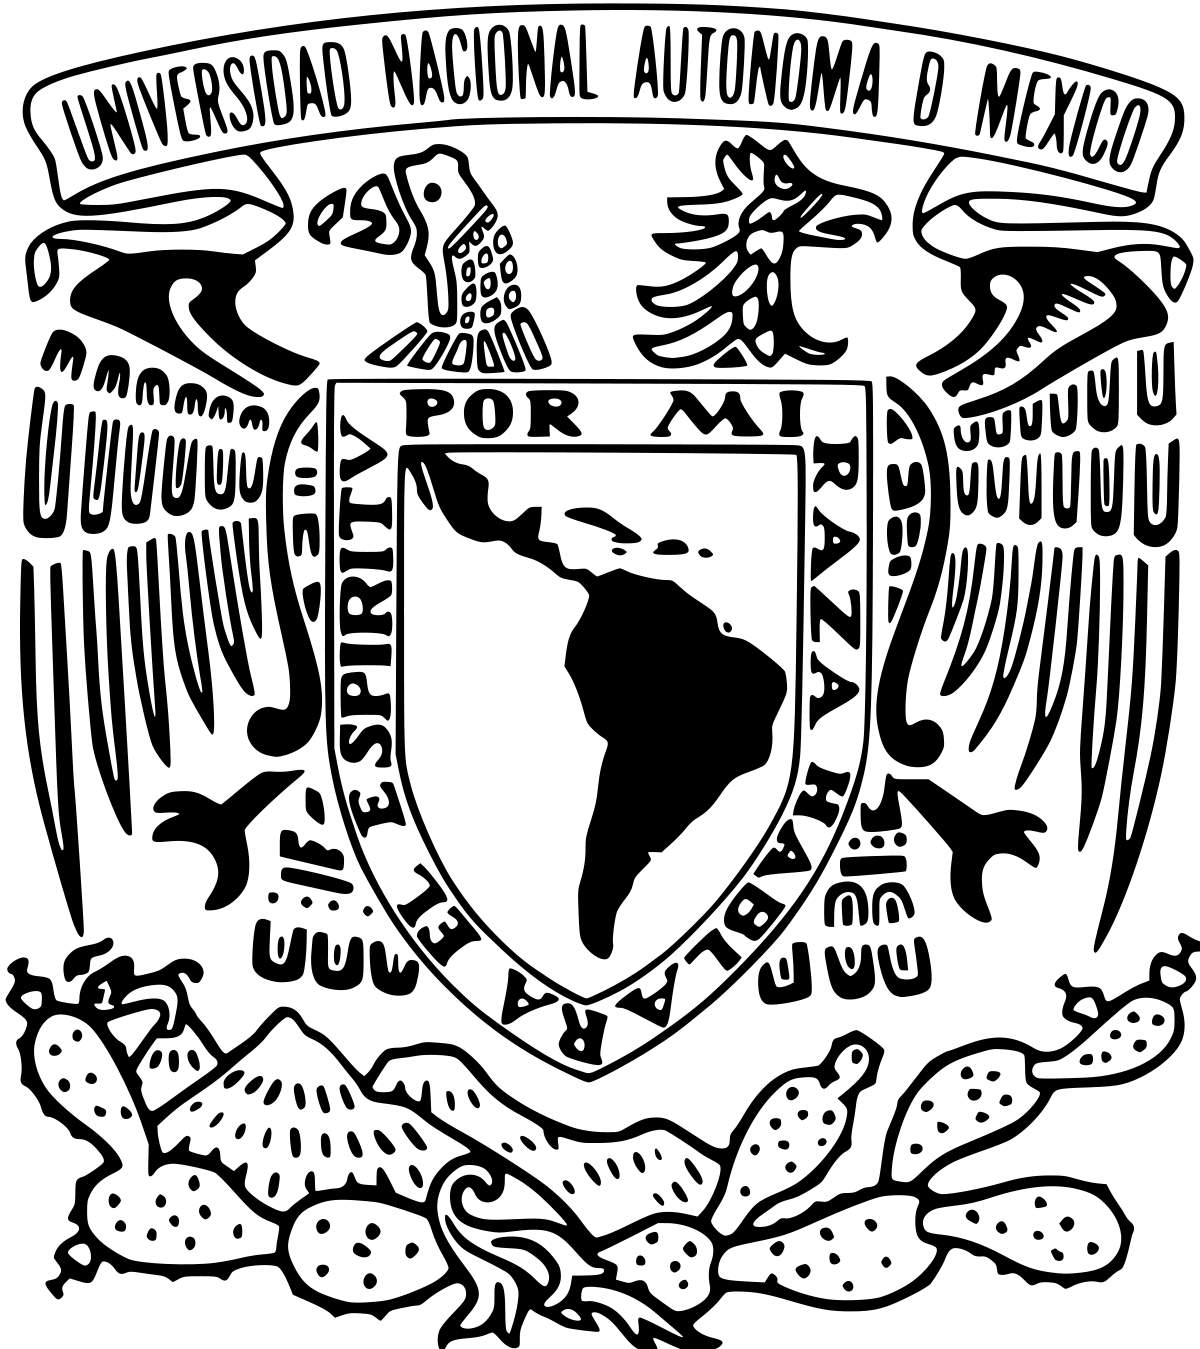
\includegraphics[width=1cm, height=1cm]{Imágenes/UNAM.png}}%%CenterHead
%\lfoot{USM}
\rhead{Estructura de Datos y Algoritmos II}%%RightHead

\setlength{\columnsep}{4mm}%Comandos para el formato de la página.
%\setlength{\parindent}{4em}%Sangría al comenzar un nuevo párrafo.
\setlength{\parindent}{0.5in}
%\setlength{\parindent}{4em}%Sangría al comenzar un nuevo párrafo.
\setlength{\parskip}{1em}%Distancia entre párrafos.
\renewcommand{\baselinestretch}{1.0}% Espacio entre línea y línea.
\setlength{\headheight}{33pt}

%Fin formato de Página

\begin{document}
  \newpage
    \tableofcontents
      \newpage


\section{Objetivos}
\begin{itemize}

\item Que el alumno implemente los algoritmos de ordenamiento externos y que conozca los elementos para el manejo de archivos.
\item Que el alumno aplique los conceptos generales de programación.
\item Que el alumno desarrolle sus habilidades de trabajo en equipo.

\end{itemize}

\pagebreak

\section{Introducción}
 \noindent De manera constante en la solución de problemas en programación es necesario manejar grandes cantidades de datos de forma eficiente, Dichas cantidades de información crecen con el paso del tiempo, como claro ejemplo tenemos el Big Data. Las técnicas necesarias para lograrlo se han ido desarrollando conforme las necesidades surgen en la solución de problemas, una de las técnicas para lidiar con la gran cantidad de información, son los algoritmos de ordenamiento.
 
Se sabe que el ordenamiento permite una mejor gestión de la información, pero, ¿qué es el ordenamiento? Es una una operación que consiste en reacomodar colecciones de datos de tal manera que sigan un orden lógico o una secuencia, siguiendo algún criterio, ascendente o descendente, por ejemplo.

Para efectos del presente proyecto, se tratarán tres algoritmos de ordenamiento externo: Poliface, Mezcla equilibrada y Radix externo. Se tratarán por separado con la intención de dejar lo más claro posible cada uno de los algoritmos y de esta manera permitir que los estudiantes adquieran de manera significativa conocimientos sobre estos algoritmos.

\pagebreak

\section{Marco Teórico}

\noindent A largo del desarrollo de las bases de datos, solució de problemas en programación y otras cuestiones que tengan que ver con el uso de grandes cantidades de datos, se han implementado algoritmos de ordenamiento.

Los algoritmos de ordenamiento más conocidos son: Insertion sort, Selection Sort, Heap Sort, Bubble Sort, Quick Sort, Counting Sort, Radix Sort y Merge Sort.
Los algoritmos de ordenamiento tienen 4 operaciones fundamentales: 
\begin{itemize}

\item Comparación            
\item Intercambio 
\item Intercalación           
\item Inserción

 
\end{itemize}

Ahora, si bien todos los algoritmos son capaces, en teoría, de ordenar una colección de N elementos, en la práctica se tiene un inconveniente que se presenta cuando la colección es muy grande y la memoria interna (RAM) no es capaz de soportar o manejar todos los datos al mismo tiempo, ya que la memoria no es infinita. Antes se trabajaba solo  de manera interna y los datos se  tenian que manejar en una sola ejecución, por lo que cuando la memoria interna es incapaz de mantener todos los datos al mismo tiempo, el algoritmo inevitablemente fallaría en estos caos.

 A medida que pasa el tiempo la cantidad de datos que deben ser ordenados crece con rápidez mayor a la que se desarrollan computadoras con mayor capacidad de almacenamiento, es en este punto donde surge la necesidad de emplear algoritmos de ordenamiento externo. Los cuales se auxilian de componentes externos para almacenar los elemento a ordenar y de esta manera optimizar la manera el la que se manejan los datos a ordenar.

Los algoritmos de ordenamiento externo se basan en la estrategia divide y vencerás, la cual permite la construcción de subproblemas menos complejos  a partir del problema general  con el objetivo de facilitar el  manejo de la información de el problema y de esta forma hacer más eficiente la solución de el problema general.

Los algoritmos de ordenamiento que se tratarán en el presente documento son todos externos, es decir, es necesario emplear memoria adicional y archivos, los cuales funcionarán como apoyo para aplicar la estrategia con la que están diseñados estos algoritmos. 

\subsection{Polifase}

Este algoritmo utiliza tres archivos adicionales al archivo que contiene la colección de datos a ordenar.

La manera en que realiza las particiones se basa en bloques de un tamaño fijo, la longitud de los bloques queda predefinida según lo que se requiera en el programa. Los bloques de longitud M serán leídos de un archivo $F_{0}$, posteriormente cada bloque se reescribirá de forma intercalada en el los archivos auxiliares:  el primer bloque irá a $F_{1}$ y el segundo a $F_{2}$, y así sucesivamente.

Una vez que no haya más bloques que reescribir, empezarán a intercalarse entre ellos, para dar lugar a bloques del doble de tamaño, dichos bloques se escribirán en los archivos $F_{0}$ y $F_{3}$ de manera intercalada, de forma similar a como se escribieron en $F_{1}$ y $F_{2}$.

Las acciones antes mencionadas se repetirán hasta que ya no sea posible general bloques de mayor tamaño. Cuando esto suceda, la colección de datos quedará ordenada.

Ejemplo:

Dado el archivo $F_{0}= {12,34,87,56,19,43,65,78,12,34,23,45,67,89,76,12,56,43,78,89}$ y M=3, se realizarán las siguientes acciones:

$F_{1} = { [12,34,87], [12,65,78], [67,76,89], [78,89] }$

$F_{2} = { [19,43,56], [23,34,45], [12,43,56] }$

Como se puede ver el $F_{1}$, no siempre se logran hacer bloque del tamaño especificado, el último bloque con frecuencia es de menor tamaño.

Una vez obtenidos esos archivos, empiezan a mezclarse los bloques de manera que se vayan ordenando al momento de escribirse en el archivo correspondiente, se escribe en $F_{0}$ y $F_{3}$ de la siguiente forma.
$F_{0} = { [ 12,19,34,43,56,87 ], [ 12,43,56,67,76,89 ]}$

$F_{3} = {[ 12,23,34,45,65,78 ], [ 78,89 ] }$

En caso de no haber otro bloque con el cual combinar el último bloque esté pasa tal cual al archivo que corresponda.

Ser repite el proceso las veces necesarias, hasta que ya no sea posible formar bloques de mayor tamaño.

$F_{1} = { [12,12,19,23,34,34,43,45,56,65,78,87 ] }$

$F_{2} = { [ 12,43,56,67,76,78,89,89 ] }$

$F_{0} = { [12,12,12,19,23,34,34,43,43,45,56,56,65,67,76,78,78,87,89,89 ] }$


La colección ha sido ordenada.

\subsection{Mezcla Equilibrada}

Este algoritmo también recibe el nombre de Mezcla Natural, trabaja de manera similar a Polifase, las diferencias entre estos dos algoritmos son:


\begin{itemize}

\item Polifase trabaja con bloque de tamaño fijo y predefinido, mientras Mezcla Equilibrada lo hace con bloques de tamaño variable. Esto debido a que al trabajar con mezcla equilibrada los bloques que se tomen serán de tamaño máximo, tomando com criterio que los elementos de cada bloque estarán ordenados según el criterio deseado para toda la colección de datos. De ahí surge otra diferencia con Poliface, no es necesario emplear un algoritmo de ordenamiento interno, pues los bloque para Mezcla Equilibrada ya están ordenados desde el momento en el que fueron formados.

\item Polifase requiere tres archivos adicionales, por su parte Mezcla Equilibrada requiere únicamente dos.

\end{itemize}

Ejemplo:

Si utilizamos la misma colección del ejemplo de Polifase:

 $F_{0}= {12,34,87,56,19,43,65,78,12,34,23,45,67,89,76,12,56,43,78,89}$
 
obtenemos:

$F_{1} { [ 12,34,87 ], [ 19,43,65,78 ], [ 23,45,67,89 ], [ 12,56 ] }$

$F_{2} = { [56], [ 12,34 ] ,[ 76 ], [ 43,78,89 ] }$

Una vez repartidos los bloques entre esos dos archivos, se hace la combinación de los elementos en el archivo F0 de la siguiente forma.

$F_{0} = { [ 12,34,56,87 ], [ 12,19,34,43,65,78 ], [ 23,45,67,78,89,89 ], [ 12,43,56,78,89 ] }$

Aquí termina la primera iteración y a partir de estos nuevos bloques se generarán otros bloques de mayor tamaño.

$F_{1} = {  [ 12,34,56,87 ],  [ 23,45,67,78,89,89 ]}$

$F_{2} = { [ 12,19,34,43,65,78 ],  [ 12,43,56,78,89 ] }$

$F_{0} = { [ 12,12,19,34,34,43,56,78,87 ], [ 12,23,43,45,56,67,78,78,89,89,89 ] }$

Fin de la segunda iteración.

$F_{1} = { [ 12,12,19,34,34,43,56,78,87 ] }$

$F_{2} = { [ 12,23,43,45,56,67,78,78,89,89,89  ] }$

$F_{0} = { [ 12,12,12,19, 23, 34, 34, 43, 43, 45, 56, 56, 67, 78, 78, 78, 87, 89, 89. 89 ] }$

Fin de la tercera iteración y fin del algoritmo, ya que no es posible formar bloques de mayor tamaño y la colección ya está ordenada.


\subsection{Radix Externo}

En el caso de este algoritmo la forma en que se realizan las particiones cambia con respecto a cómo se han hecho en Polifase y Mezcla Equilibrada.

Está vez las particiones se hacen en base a los dígitos significativos de cada uno de los elementos de que deben ser ordenados. 

Por lo general este algoritmo requiere de más archivos auxiliares en comparación con los algoritmos antes mencionados, la cantidad de estos dependen de los posibles dígitos distintos que tengan las claves a ordenar. Es necesario un archivo por cada uno de los posibles dígitos que contengan  las claves.

Es necesario aclarar que cuando se habla de dígitos se contemplan los números, las letras y otros caracteres que puedan componer a las claves.

Ejemplo: 

Si se tiene el archivo $F_{*} = { 234,241,421,342,32,443,112,34,432,13 }$

Los archivos necesarios serán: $F_{0}$ = ,$F_{1}$ = , $F_{2}$ = , $F_{3}$ = , $F_{4}$ =

Un archivo por cada dígito diferente: 0,1,2,3 y 4.

Una vez teniendo esto claro, se inicia tomado el dígito menos significativo, que en este caso como son números, se toman las unidades:

\noindent$F_{0}  = {  } $

$F_{1} = { 241, 421 }$

$F_{2} = {  342, 32, 112, 432  }$
$F_{3} = { 443, 13 }$

$F_{4} = { 234, 34 }$

En este caso, como se ordenarán de forma ascendente, primero se “vacía” el archivo correspondiente al dígito con menor valor y el último que se vacía será el del dígito con mayor valor.

Se sobreescribe en el archivo que tenía las claves en el orden original de manera que se respete la regla  con la que se desea ordenar la colección completa en este caso de manera ascendente.

Es importante resaltar que los archivos que se usarán para dividir las claves se comportan de manera similar a una estructura FIFO (First In First Out).

$F_{*} = { 241, 421, 32, 112, 342, 432, 13, 443, 34, 234 }$

Se sigue con la división de las claves en los archivos, pero ahora se toma en cuenta el siguiente dígito más significativo que el anterior: las decenas. De la siguiente manera.

$F_{0} = {  }$

$F_{1} = { 112, 13 }$

$F_{2} = { 421 }$

$F_{3} = { 32, 432, 34, 234 }$

$F_{4} = { 241, 342, 443 }$

$F_{*} = { 112,13,421,32,432,234,34,241,342,443 }$

Se sigue con la división de las claves en los archivos, pero ahora se toma en cuenta el siguiente dígito más significativo que el anterior: las centenas. De la siguiente manera.

$F_{0} = { 13,32,34 }$

$F_{1} = { 112 }$

$F_{2} = { 234,241 }$

$F_{3} = { 342 }$

$F_{4} = { 421, 432,443 }$

$F_{*} = { 13,32,34,112,234,241,342,421,432,443 }$

Dado que ya no hay más dígitos significativos que clasificar, el algoritmo llega a su fin y da como resultado la colección ya ordenada.

\pagebreak

\section{Metodología de desarrollo}

\subsection{Entorno inicial de trabajo}
    
\noindent La programación de una solución al problema del ordenamiento de claves con 3 campos requiere abstraer y dividir el problema inicial en 3 sub-problemas:

\begin{itemize}
\item Almacenar cada una de las claves en estructuras de datos auxiliares.

\item Leer archivos y escribir sobre ellos.

\item Generar nuevos archivos o eliminarlos. 

\end{itemize}
    
\subsection{Lectura y escritura de archivos en Java}

\noindent \textbf{Java} posee diversas clases que permiten la apertura, así como la lectura y escritura en archivos existentes:

\begin{itemize}
\item La clase \textit{File} permite crear un objeto que tiene asociado al archivo que se desea manipular; estableciendo la ruta de acceso al archivo en el constructor del objeto. 

\begin{figure}[h!]
\centering
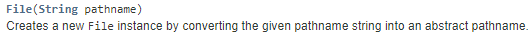
\includegraphics[height=1cm]{Imágenes/Met1.png}
\caption{\textit{Constructor básico de File.}}
\label{fig:Met1}
\end{figure}


\item La clase \textit{FileReader} permite inicializar un proceso de lectura sobre un objeto de tipo \textit{File}; introduciendo en el constructor un objeto inicializado de tipo \textit{File}, respectivamente. Su uso está pensado específicamente para la lectura de archivos con caracteres.

\begin{figure}[h!]
\centering
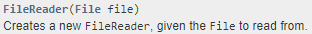
\includegraphics[height=1cm]{Imágenes/Met2.png}
\caption{\textit{Constructor básico de FileReader.}}
\label{fig:Met2}
\end{figure}

\item Las herramientas proporcionadas por la clase \textit{BufferedReader} permiten una lectura eficiente de caracteres, arreglos y líneas generando un \textit{buffer} que almacena los datos temporalmente y agiliza el proceso de lectura de archivos externos. Al crear un objeto de esta clase, su constructor debe incluir como parámetro un objeto de tipo \textit{FileReader}.

\begin{figure}[h!]
\centering
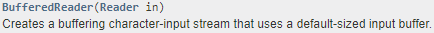
\includegraphics[height=1cm]{Imágenes/Met3.png}
\caption{\textit{Constructor básico de BufferedReader.}}
\label{fig:Met3}
\end{figure}

\item La clase \textit{FileWriter} permite inicializar un proceso de escritura sobre un objeto de tipo \textit{File}; introduciendo en el constructor un objeto inicializado de tipo \textit{File}, respectivamente. Su uso está pensado específicamente para la escritura de caracteres.

\begin{figure}[h!]
\centering
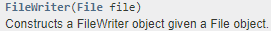
\includegraphics[height=1cm]{Imágenes/Met4.png}
\caption{\textit{Constructor básico de FileWriter.}}
\label{fig:Met4}
\end{figure}

\item Las herramientas proporcionadas por la clase \textit{BufferedWriter} permiten una escritura eficiente de caracteres, arreglos y líneas generando un \textit{buffer} que almacena los datos temporalmente y agiliza el proceso de escritura de caracteres sobre archivos externos. Al crear un objeto de esta clase, su constructor debe incluir como parámetro un objeto de tipo \textit{FileWriter}.

\begin{figure}[h!]
\centering
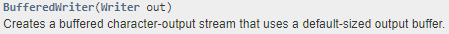
\includegraphics[height=1cm]{Imágenes/Met5.png}
\caption{\textit{Constructor básico de BufferedWriter.}}
\label{fig:Met5}
\end{figure}

\end{itemize}

El uso de cada una de las clases anteriores requiere el manejo de \textbf{Excepciones}: mensajes de error asociados a entradas incorrectas, defectos en el código de un programa o errores de diseño. Cuando un error de esta naturaleza se presente, \textbf{Java} terminará inmediatamente la ejecución del programa e imprimirá en pantalla un mensaje de error.

Para manejar internamente las excepciones, se requiere el uso de las líneas \textbf{try - catch}:

\begin{itemize}

\item La declaración \textbf{try} permite definir un bloque de código que será puesto a prueba, verificando que no existan errores mientras se ejecuta.

\item La declaración \textbf{catch} permite definir un bloque de código que se ejecutará únicamente en caso de que se detecte un error en el bloque de código definido por \textbf{try}.

\end{itemize}

\begin{figure}[h!]
\centering
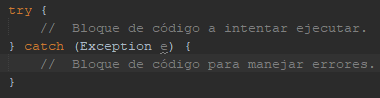
\includegraphics[height=3cm]{Imágenes/Met6.png}
\caption{\textit{Estructura try-catch.}}
\label{fig:Met6}
\end{figure}

\subsection{Generación de archivos}

\noindent Crear nuevos archivos a través de la clase \textit{File} es una tarea sencilla. Al momento de inicializar un objeto de tipo \textit{File} con una ruta de acceso especificada y un nombre, la clase permite utilizar 2 métodos: \textbf{exists()} y \textbf{createNewFile()}. A través de estos 2 métodos se puede verificar si existe o no un archivo y, en caso de que no exista, crearlo en la ruta establecida en el objeto \textit{File}.

\begin{figure}[h!]
\centering
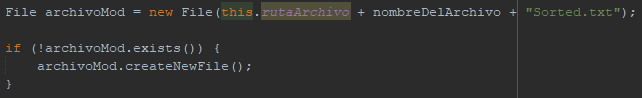
\includegraphics[height=2.3cm]{Imágenes/Met7.png}
\caption{\textit{Generación de un archivo no existente.}}
\label{fig:Met7}
\end{figure}


\subsection{Lectura inicial de las claves}

\noindent Una de las partes vitales de la implementación del ordenamiento externo reside en obtener una solución eficaz a la lectura y carga de las claves solicitadas, las cuales están compuestas cada una de 3 campos: Nombre, Apellido y Número de Cuenta. Con fin de identificar internamente las claves a manipular en el programa, las claves con sus 3 campos serán denominadas \textbf{superclaves} y cada campo se denominará como una \textbf{subclave}. 

La solución al problema, por tanto, requiere del uso de un arreglo dinámico anidado que contega cada \textbf{superclave} en cada uno de sus índices, y a su vez, cada superclave represente otro arreglo que contenga cada una de las \textbf{sub-claves} que la componen. 

Uno de los métodos creados para el proyecto denominado \textbf{scanSuperKeys} brinda una solución a tal problema, generando un arreglo multidimensional anidado que guardará cada una de las superclaves y sus respectivas subclaves. El resultado final, por tanto, se asemeja a los ejemplos teóricos analizados en el curso teórico de EDA II y permite un manejo más natural e intuitivo sobre cada una de las claves.

Los pasos que sigue este método son los siguientes:

\begin{enumerate}
\item Inicializa un arreglo anidado de cadenas de caracteres llamado \textbf{lecturaDF0} de tipo \textit{ArrayList}.

\item Carga por medio de la clase \textit{File} el archivo a leer con las claves deseadas y, posteriormente, se inicializa un objeto \textit{Scanner} introduciendo como parámetro en su constructor el objeto \textit{File} creado.

\item Mientras el escáner detecte líneas de texto en el archivo, se definirá a cada línea con el nombre \textbf{saltoClave} (Ya que cada línea de texto en el archivo contiene 1 sola superclave) y se definirá como el \textbf{identificador} de cada superclave un espacio vacío existente entre ellas por medio de la clase \textit{StringTokenizer}, que recibe una cadena y la separa al momento de leer un caracter definido como el \textbf{delimitador}.

\item A continuación, se recupera cada superclave y se inicializa otro arreglo dinámico de cadenas denominado \textbf{subClaves}.

\item Se inicializa otro objeto de tipo \textit{StringTokenizer} llamado \textbf{separador} que recibirá como parámetro cada superclave y usará como delimitador de cada subclave el carácter $","$. Posteriormente, se añadirá cada subclave a la lista utilizando el método \textbf{nextToken()} por medio de un ciclo \textbf{for}.

\item Finalmente, se añade el arreglo con las 3 subclaves en el arreglo \textbf{lecturaDF0} y se imprime el resultado en pantalla. 

\end{enumerate}

\begin{figure}[h!]
\centering
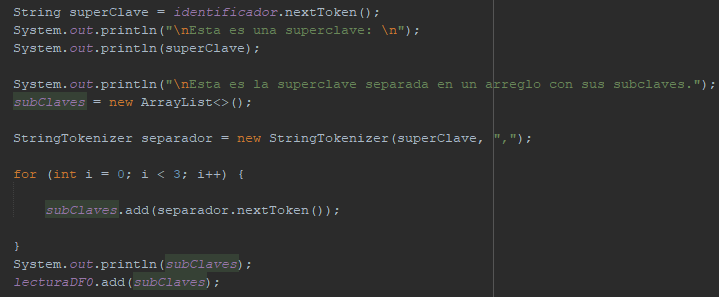
\includegraphics[height=6cm]{Imágenes/Met8.png}
\caption{\textit{Proceso de lectura y almacenamiento de cada superclave.}}
\label{fig:Met8}
\end{figure}

Con fines de prueba, se ha utilizado un archivo $.txt$ que contiene 5 superclaves con el formato especificado. Este archivo será leído por \textbf{scanSuperKeys} y lo almacenará en un arreglo dinámico anidado:

\begin{figure}[h!]
\centering
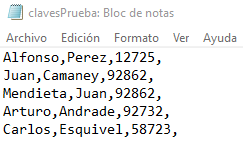
\includegraphics[height=3cm]{Imágenes/Met9.png}
\caption{\textit{Archivo con 5 superclaves.}}
\label{fig:Met9}
\end{figure}

\begin{figure}[h!]
\centering
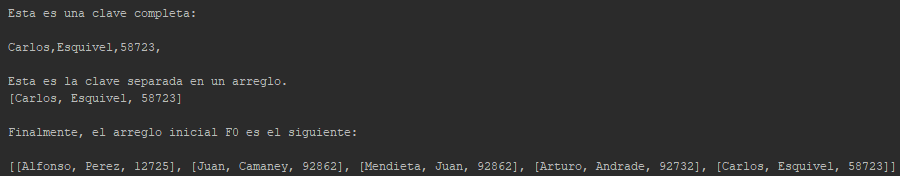
\includegraphics[height=3.5cm]{Imágenes/Met10.png}
\caption{\textit{Arreglo anidado resultante.}}
\label{fig:Met10}
\end{figure}

Al término de su ejecución, el método devuelve el arreglo anidado para que cualquier método de ordenamiento que lo invoque pueda hacer uso del mismo; teniendo un acceso sencillo a cada una de las subclaves de acuerdo al campo de ordenamiento que se desee utilizar (Ordenamiento por Nombre, Apellido o Número de cuenta).  


\section{Análisis de las implementaciones}

\subsection{Simulación de Polifase}

\subsubsection{Polifase numérica}

\noindent El primer método de ordenamiento tiene entre sus atributos las rutas de acceso a los archivos iniciales, así como los archivos auxiliares que utilizará durante su ejecución. Además, se tienen declaradas referencias a objetos de tipo \textit{BufferedReader}, \textit{BufferedWriter}, \textit{StringTokenizer} y \textit{FileWriter} y finalmente, se añaden referencias a objetos \textit{ArrayList} que serán utilizados para recuperar la lista de superclaves y manipularla.

\begin{figure}[h!]
\centering
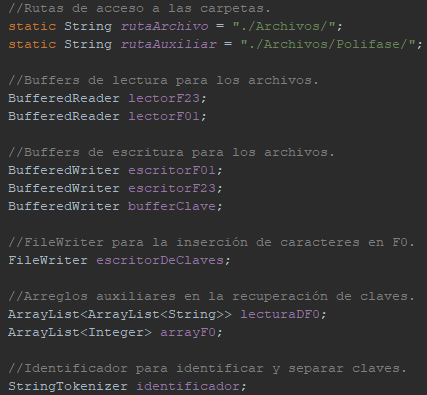
\includegraphics[height=9cm]{Imágenes/PoliN1.png}
\caption{\textit{Atributos de la clase Polifase.}}
\label{fig:PoliN1}
\end{figure}

\pagebreak

A continuación, se listarán los métodos secundarios creados para la clase \textit{Polifase}. La documentación completa de su funcionamiento se encuentra en el código fuente del proyecto creado. 

\begin{itemize}
\item \textbf{hubReader} y \textbf{hubWriter} son métodos dedicados a la creación de buffers de lectura y escritura para los archivos F0, F1, F2 y F3 durante la ejecución del programa. Su uso tiene como ventaja proporcionar una apertura rápida de flujos de lectura/escritura sobre los archivos auxiliares y, por tanto, tener un control simplificado de los buffers. Así mismo, permite obtener un código fuente más claro y limpio. 

\begin{figure}[h!]
\centering
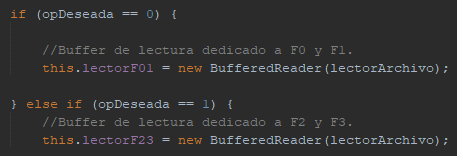
\includegraphics[height=4cm]{Imágenes/PoliN2.png}
\caption{\textit{Buffers de lectura para los archivos de Polifase.}}
\label{fig:PoliN2}
\end{figure}

\begin{figure}[h!]
\centering
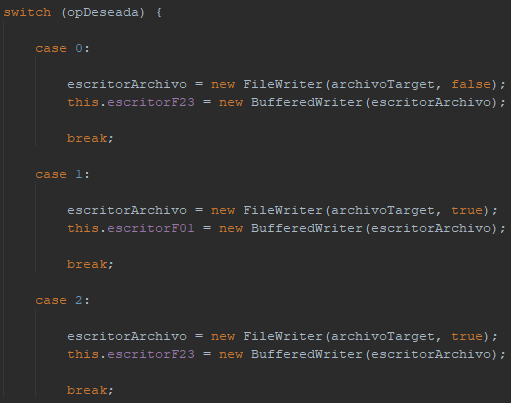
\includegraphics[height=9cm]{Imágenes/PoliN3.png}
\caption{\textit{Buffers de escritura para los archivo de Polifase.}}
\label{fig:PoliN3}
\end{figure}

\item El método \textbf{appendKeyToFile} es utilizado durante la ejecución de Polifase para añadir las subclaves recuperadas del arreglo \textbf{lecturaDF0} a un archivo $"F0"$ inicial y comenzar el ordenamiento a partir del mismo; sin alterar el archivo original con las superclaves. 

\begin{figure}[h!]
\centering
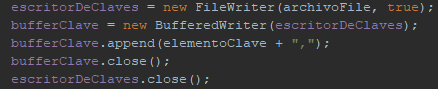
\includegraphics[height=3cm]{Imágenes/PoliN4.png}
\caption{\textit{Uso de buffers de escritura para añadir claves a un archivo.}}
\label{fig:PoliN4}
\end{figure}

\item \textbf{internalSortingArray} es utilizado durante la generación de los bloques de subclaves generados por Polifase. Cada bloque, recibido como una cadena de caracteres, es transformado a un arreglo de subclaves utilizado el método \textbf{split} definido para la clase \textit{String}; el cual funciona de forma equivalente a \textit{StringTokenizer}. Utilizando como delimitador el carácter $","$ se añade cada clave a un arreglo dinámico por medio de un ciclo \textbf{for-each}; transformando las subclaves a enteros por medio del método \textbf{parseInt} definido para el envoltorio \textit{Integer}.

Posteriormente, se utiliza el método de ordenamiento interno \textit{Insertion-Sort} definido en la clase \textit{Utilidades} sobre el arreglo dinámico. Con el arreglo ordenado, se realiza el proceso inverso, extrayendo del arreglo cada subclave ordenada y creando una cadena que, finalmente, es devuelta por el método.

\begin{figure}[h!]
\centering
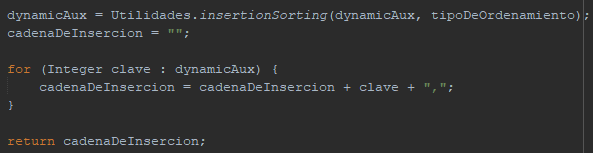
\includegraphics[height=3cm]{Imágenes/PoliN5.png}
\caption{\textit{Ordenamiento de bloques de claves.}}
\label{fig:PoliN5}
\end{figure}


\item El método \textbf{lecturaLinea} permite leer y recuperar como una cadena de caracteres el contenido presente en una línea establecida como parámetro. Este método fue generado debido a que, entre cada iteración de Polifase, se escriben 2 saltos de línea para mantener una separación entre los bloques de claves que son escritos y recuperados de forma sucesiva. 

\begin{figure}[h!]
\centering
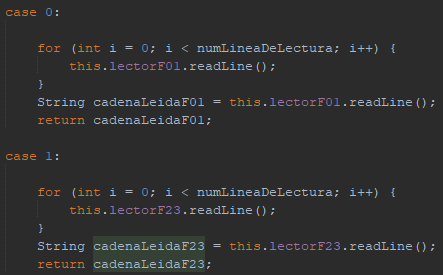
\includegraphics[height=6cm]{Imágenes/PoliN6.png}
\caption{\textit{Lectura y recuperación de líneas transformadas a cadenas de caracteres.}}
\label{fig:PoliN6}
\end{figure}

\end{itemize}

\pagebreak

Una vez establecidos los métodos secundarios, se enlistarán los 2 métodos principales de la implementación de Polifase realizada: 

\begin{itemize}
\item \textbf{ordenamientoPolifase} es el primer método inicial y es el que se invoca en el menú principal del programa. Recibiendo el nombre del archivo con las claves, el tamaño de los bloques de claves (Para efectos del proyecto, se ha establecido en 4) y el criterio de ordenamiento seleccionado, inicia invocando un recolector de basura denominado \textbf{resetArchivoAuxPolyphase} que reinializa los archivos de Polifase provenientes de anteriores ejecuciones.

\begin{figure}[h!]
\centering
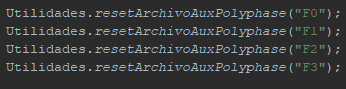
\includegraphics[height=2cm]{Imágenes/PoliN7.png}
\caption{\textit{Invocación del recolector de basura.}}
\label{fig:PoliN7}
\end{figure}

A continuación, realiza los siguientes pasos:

\begin{enumerate}
\item Recupera el arreglo anidado con las superclaves y, posteriormente, recupera la subclave 'Número de cuenta' de cada una de las superclaves y las almacena en otro arreglo dinámico; transformando en el proceso los datos a \textit{Integers} para su correcta manipulación. 

\item Por medio del método \textbf{appendKeyToFile}, se escriben cada una de las subclaves recuperadas en un archivo llamado $F_{0}$, y se inicializa un proceso de lectura sobre el archivo $F0$, así como una escritura sobre los auxiliares $F_{1}$ y $F_{2}$.

\begin{figure}[h!]
\centering
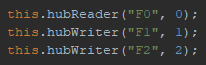
\includegraphics[height=2cm]{Imágenes/PoliN8.png}
\caption{\textit{Invocación de los hub de lectura y escritura.}}
\label{fig:PoliN8}
\end{figure}

\pagebreak

\item Se establece un primer ciclo \textbf{while} tal que, mientras el lector establecido para $F_{0}$ encuentre una cadena de claves que no sea nula, establezca un identificador de claves por medio de \textit{StringTokenizer} y un delimitador $","$. Luego, se establece por un ciclo \textbf{while} anidado que, por cada clave individual que sea recuperada, esta se almacene en un arreglo auxiliar. Mientras esta operación es realizada, un contador interno mantiene la cuenta de las claves almacenadas: cuando este valor llegue a 4, se imprime el bloque leído y se reinicializa el contador. 

\begin{figure}[h!]
\centering
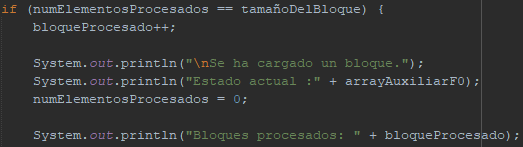
\includegraphics[height=4cm]{Imágenes/PoliN9.png}
\caption{\textit{Generación de los bloques de subclaves.}}
\label{fig:PoliN9}
\end{figure}

\item El contador \textbf{bloqueProcesado} se utiliza para enviar a $F_{1}$ o a $F_{2}$ el bloque cargado. Por ejemplo, para el primer bloque: $bloqueProcesado=1$, usando la operación $bloqueProcesado$ $mod$ $2$, si el resultado $\neq$ $0$, eso indica la presencia de un bloque impar que deberá ser enviado al archivo $F_{1}$. En cambio, si $bloqueProcesado$ $mod$ $2$ $=$ $0$, el bloque cargado es par y será enviado al archivo $F_{2}$; previamente transformado a una cadena de caracteres por medio de un ciclo \textbf{for-each} y ordenado por el método \textbf{internalSortingArray}.

\begin{figure}[h!]
\centering
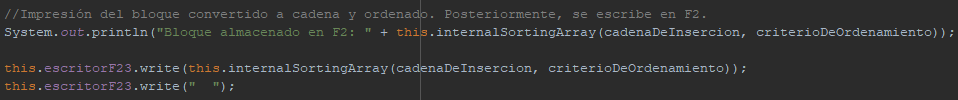
\includegraphics[height=2cm]{Imágenes/PoliN10.png}
\caption{\textit{Inserción de un bloque impar sobre .}}
\label{fig:PoliN10}
\end{figure}

\item Posteriormente, se verifica que sobre el arreglo auxiliar no existan subclaves adicionales que no alcancen el tamaño del bloque establecido. En caso de que suceda tal situación, el proceso anterior se repite, con la diferencia de que, por ejemplo, si la lectura de bloques con el tamaño establecido terminó en $F_{1}$, el contador \textbf{bloqueProcesado} tendrá con un valor impar y, por tanto, el bloque restante será enviado a $F_{2}$.

\begin{figure}[h!]
\centering
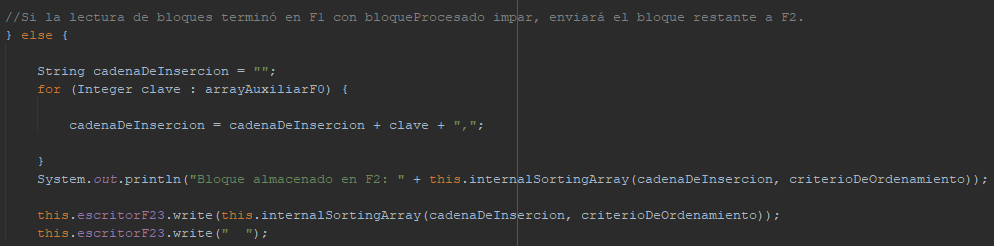
\includegraphics[height=4.5cm]{Imágenes/PoliN11.png}
\caption{\textit{Inserción de bloques con tamaño menor al establecido.}}
\label{fig:PoliN11}
\end{figure}

\item Finalmente, se cierran cada uno de los buffers de lectura/escritura utilizados y se inicializa un proceso de lectura sobre $F_{0}$ para proceder al segundo método principal del ordenamiento: \textbf{mergingPolyphase}.

\end{enumerate}


\item El método \textbf{mergingPolyphase} únicamente recibe como parámetro el criterio de ordenamiento seleccionado por el usuario. A continuación, realiza los siguientes pasos:

\begin{enumerate}
\item Inicializa por medio del método \textbf{hubReader} y \textbf{hubWriter} un proceso de lectura sobre los bloques de claves presentes en los archivos $F_{1}$ y $F_{2}$ y prepara un proceso de escritura en los archivos $F_{0}$ y $F_{3}$. Por medio de un ciclo \textbf{do-while}, se recuperan las claves presentes en la línea de lectura actual de la iteración (Recordando que, entre cada iteración de bloques escritos en los archivos, se añaden 2 espacios en blanco) y se imprimen en pantalla. Posteriormente, los bloques de claves son separados por medio del método \textbf{split} usando como identificador el espacio presente entre cada bloque de claves. 

\begin{figure}[h!]
\centering
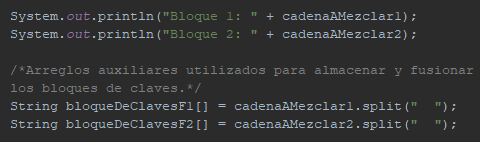
\includegraphics[height=3cm]{Imágenes/PoliN12.png}
\caption{\textit{Recuperación de bloques de clave.}}
\label{fig:PoliN12}
\end{figure}

\item Debido a la naturaleza de la generación de particiones de Polifase, existe la posibilidad de que el segundo arreglo generado en [\ref{fig:PoliN12}] sea
de menor tamaño (Contiene menor cantidad de bloques que ). Por tanto, implica que su manipulación y mezcla por medio de un ciclo \textbf{for} inevitablemente resultaría en una excepción de índice inexistente. Para evitar tal situación, se añade un bloque \textit{placeholder} al segundo arreglo en caso de que este sea de menor tamaño que el primer arreglo. De esta forma, se asegura que ambos arreglos sean siempre del mismo tamaño.

\begin{figure}[h!]
\centering
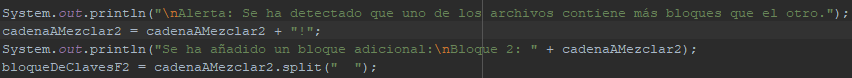
\includegraphics[height=1.7cm]{Imágenes/PoliN13.png}
\caption{\textit{Verificación y modificación sobre el segundo arreglo.}}
\label{fig:PoliN13}
\end{figure}

Durante el proceso de intercalado de ambos bloques, el bloque \textit{placeholder} es eliminado por el método \textbf{internalSortingArray}.


\item Hecho lo anterior, se inicializa un ciclo \textbf{for} que, considerando el valor de la variable \textbf{bloquesProcesados} (la cuál indica el número de bloques que han sido intercalados), escribirá sucesivamente sobre $F_{0}$/$F_{3}$ o $F_{1}$/$F_{2}$, según corresponda. 

\begin{figure}[h!]
\centering
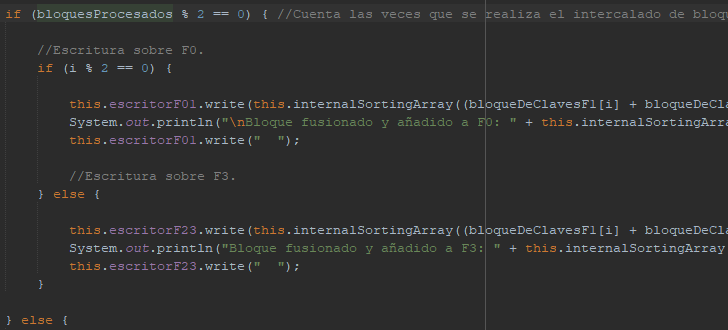
\includegraphics[height=6cm]{Imágenes/PoliN14.png}
\caption{\textit{Escritura de bloques intercalados y ordenados por medio de Insertion-Sort.}}
\label{fig:PoliN14}
\end{figure}

\item Una vez hecho la escritura intercalada de los bloques, se añaden 2 saltos de línea en los archivos y se cierran los escritores utilizados. Posteriormente, se verifica si los bloques procesados se escribieron sobre $F_{0}$/$F_{3}$ o $F_{1}$/$F_{2}$ para inicializar su lectura y repetir el proceso de intercalado sobre el otro par de archivos auxiliares.

En caso de que se detecte que alguna de las cadenas de bloques recuperadas no contiene elementos, se rompe el ciclo \textbf{while} y se indica en pantalla que los datos han sido finalmente ordenados. 

\begin{figure}[h!]
\centering
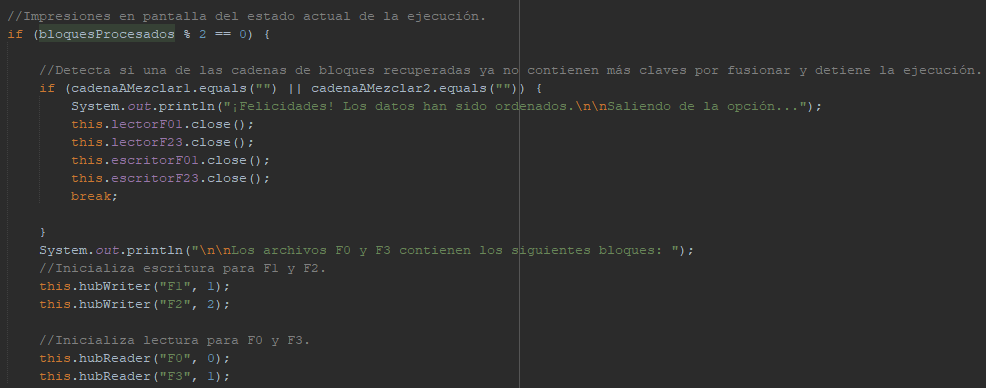
\includegraphics[height=6.5cm]{Imágenes/PoliN15.png}
\caption{\textit{Condición de ruptura del ciclo while e inicialización de escritura sobre $F_{1}$/$F_{2}$.}}
\label{fig:PoliN15}
\end{figure}


\end{enumerate}

\end{itemize}


\pagebreak


\subsubsection{Polifase no numérica}

\noindent El ordenamiento de claves no numéricas contiene diferencias con respecto al enfoque numérico, por tanto, su implementación se encuentre contenida sobre otra clase que hereda directamente de \textit{Polifase}: a esta clase se le ha denominado \textit{PolifaseStrings}. A continuación se mostrarán las diferencias con respecto a la implementación anterior. 

Se crea un arreglo el cual contendrá nuestras de claves de tipo String para almacenar claves no numéricas, como los nombres o apellidos.

\begin{figure}[h!]
\centering
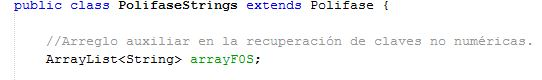
\includegraphics[height=2.5cm]{Imágenes/PolifaseN1.png}
\caption{\textit{Arreglo auxiliar en la recuperación de claves no numericas.}}
\label{fig:PolifaseN1}
\end{figure}

La recuperación de las claves presenta modificaciones: debido a que es posible seleccionar entre Nombre o Apellido, con valor (1) o (2) respectivamente durante la selección del campo en el menú principal, se obtendrán las claves de acuerdo al campo que fue escogido, restando $-1$ tomando en consideración el índice inicial del arreglo siendo 0.

\begin{figure}[h!]
\centering
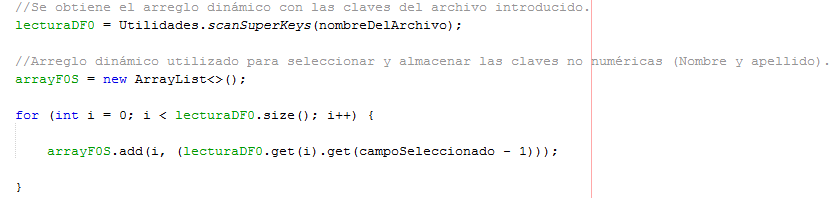
\includegraphics[height=4cm]{Imágenes/PolifaseN3.png}
\caption{\textit{Recuperación de claves no numéricas.}}
\label{fig:PolifaseN3}
\end{figure}

El ciclo de lectura y generación de bloques es modificado para adaptarse a la lectura de claves no numéricas. El resto del procedimiento se mantiene sin cambios.


\begin{figure}[h!]
\centering
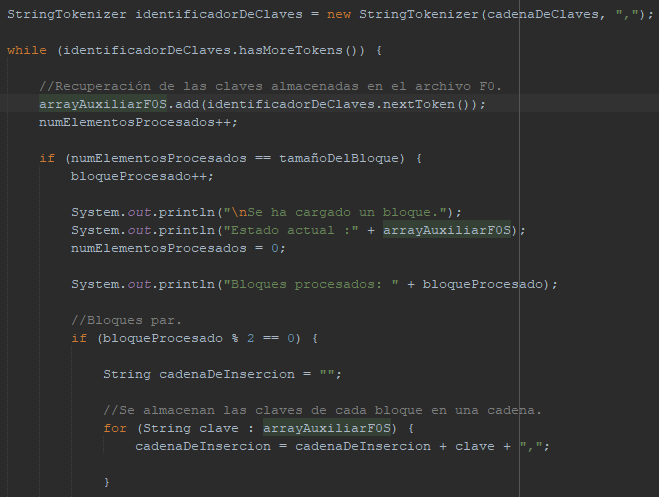
\includegraphics[height=11cm]{Imágenes/PolifaseN5.png}
\caption{\textit{Ciclo de lectura de claves y almacenado en un arreglo auxiliar.}}
\label{fig:PolifaseN4}
\end{figure}

\pagebreak

El método \textbf{internalSortingArray} es modificado para admitir el ordenamiento de claves no numéricas. El resto del procedimiento, sigue sin cambios adiciones; más allá de las modificaciones a los ciclos \textbf{for-each} implementados que iterarán sobre Strings.

\begin{figure}[h!]
\centering
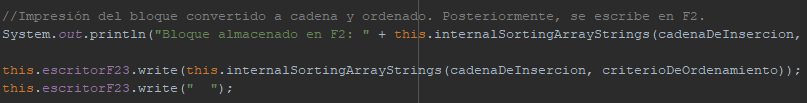
\includegraphics[height=2cm]{Imágenes/PolifaseN7.png}
\caption{\textit{Ciclo para lectura de claves y guardarlas en los arreglos dinamicos.}}
\label{fig:PolifaseN7}
\end{figure}

\pagebreak

El método \textbf{mergingPolyphaseString} es una modificación de \textbf{mergingPolyphase} adaptado al procesamiento de claves no numéricas. En general, el cambio más significativo reside en el uso del método modificado \textbf{internalSortingArrayStrings} que permite ordenar claves no numéricas. Así mismo, el resto de métodos han sido adaptados para procesar claves de tipo String.

\subsection{Simulación de Radix Externo}

\noindent Los atributos de la clase que se utilizará para este algoritmo incluyen:

\begin{itemize}

   \item Las rutas donde se encontrarán los archivos utilizados para la implementación de este algoritmo de ordenamiento externo.
   
   \item Elementos para escribir las claves a ordenar.
   
   \item Elementos para leer las claves a ordenar.
   
   \item Un arreglo auxiliar para leer las claves de archivo $_F{0}$, el cual será de tipo ArrayList con elementos tipo ArrayList de cadenas de caracteres.
   
\end{itemize}

\begin{figure}[h!]
\centering
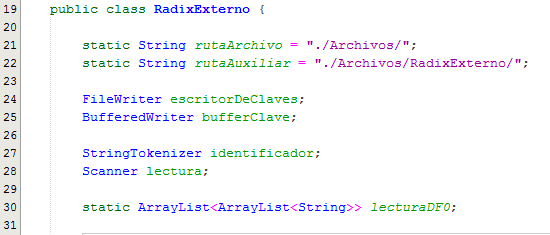
\includegraphics[height=5cm]{Imágenes/AtributosRadix.PNG}
\caption{\textit{Atributos de Radix Externo.}}
\label{fig:RadN1}
\end{figure}

Así mismo la clase cuenta con varios métodos para la implementación de este algoritmo. A continuación, se dará una vista general de ellos; la documentación completa puede ser consultada en el código de la clase RadixExterno.java

\begin{itemize}
    \item\textbf{ordenamientoRadix}
    
    Este primer método es el método principal de Radix, recibe 2 parametros, el primero es el nombre del archivo que contiene la claves que deben ordenarse el cual no es el original, es más bien una copia, esto e hizo con el propósito de no modificar el archivo original para poder hacer más ejecuciones posteriormente. El segundo parámetro es el criterio que se utilizará para hacer el ordenamiento, ya sea ascendente o descendente, según lo indique el usuario..

    Este método posee un contador de iteraciones para que el usuario pueda hacer el seguimiento de los pasos que hace el algoritmo.
    
    Contempla posibles errores de escritura, los evita borrando algunos archivos o limpiandolos para que no haya problemas por corridas anteriores.
    
    Así mismo, crea e indica las posiciones significativas que el algoritmo va tomando en cuenta conforme realiza el ordenamiento.
    
    Uno de los aspectos relevante es el uso de simulaciones de estructuras de tipo FIFO que contribuyen al ordenamiento mediante este algoritmo, se habla de una simulación debido a que no se declara como tal una FIFO, pero la manera en la que se leen la claves es similar a como se haría en una estructura FIFO, los detalles sobre la creación de estas se explicará más adelante en \textbf {queueBuilder1k} y \textbf {queueBuider}
    
    \begin{figure}[h!]
    \centering
    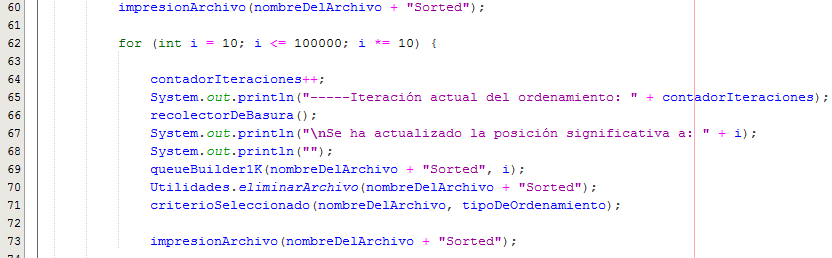
\includegraphics[height=5.5cm]{Imágenes/RaMe1.PNG}
    \caption{\textit{Método principal.}}
    \label{fig:RaMe1}
    \end{figure}
    
    \item\textbf{criterioSeleccionado}
    
    Para este método es necesario obtener dos parámetro: nombre del archivo donde se encuentran las claves ordenar para leer las claves y el tipo de ordenamiento para establecer el orden de los archivos auxiliares.

    Hace una llamada al método \textbf {sortAux} que se explicará más adelante.

    
    \begin{figure}[h!]
    \centering
    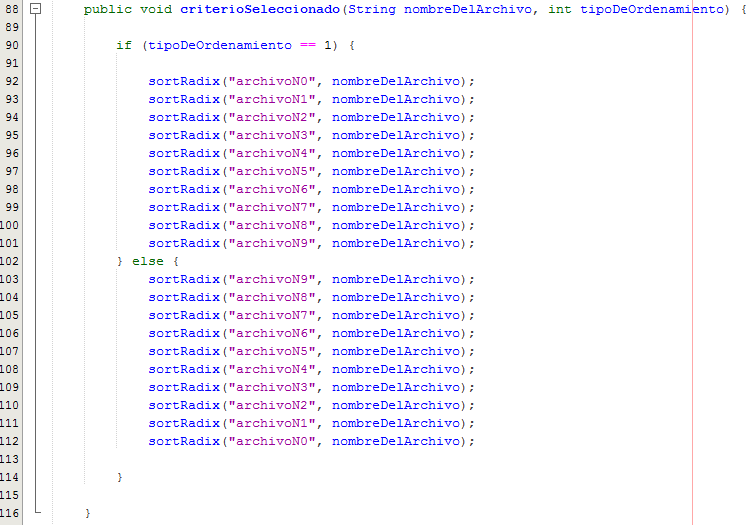
\includegraphics[height=10cm]{Imágenes/RaMe2.PNG}
    \caption{\centering\textit{Establece el orden de creación de los archivos auxiliares dependiendo del criterio de ordenamiento que el usuario seleccionó.}}
    \label{fig:RaMe2}
    \end{figure}
    
    \item\textbf{queueBuilder1K}
    
    Clasifica las claves para para asignarla al archivo auxiliar correspondiente, lo logra haciendo la lectura del archivo donde se encuentran las claves a ordenar. Es necesario utilizar otro método de la misma clase \textbf {RadixExterno.java} llamado \textbf {escrituraAuxiliar} para escribir las claves obtenidas en los archivos auxiliares según corresponda. Puede diferenciar cuando una clave termina porque toma en cuenta cuando encuentra comas \textit {“,”}
    
    Este método se usa para leer claves de los archivo que se van generando conforme se avanza en los dígitos significativos, hay un método similar a el llamado \textbf {queueBuilder}, descrito más adelante.
    
    \pagebreak
    
    \begin{figure}[h!]
    \centering
    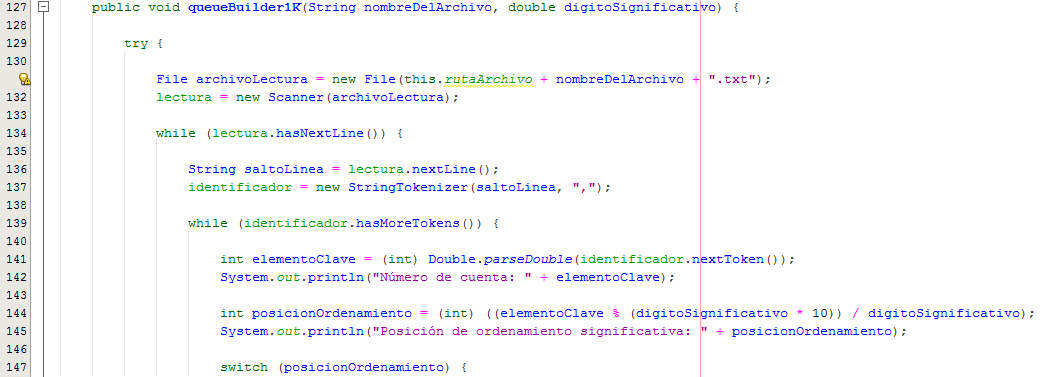
\includegraphics[height=7cm]{Imágenes/RaMe3.PNG}
    \caption{\textit{Clasifica las claves desde la iteración segunda en adelante.}}
    \label{fig:RaMe3}
    \end{figure}
    
    \item\textbf{queueBuilder}
    
    A diferencia de método anterior \textbf {queueBuilder1K} este método sólo se utiliza en la primera iteración, por ello recibe como primer parámetro el arreglo en  el que estarán las claves al leer el archivo original.

    Como segundo parámetro recibe el dígito significativo, con base a esto clasifica las claves que va obteniendo del archivo que recibe como primer parámetro. Los escribe con ayuda del método \textbf {escrituraAuxiliar}.
    
    \begin{figure}[h!]
    \centering
    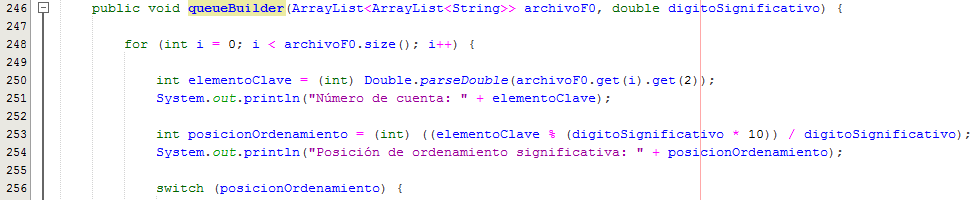
\includegraphics[height=3cm]{Imágenes/RaMe4.PNG}
    \caption{\textit{Clasifica las claves en la primera iteración.}}
    \label{fig:RaMe4}
    \end{figure}

     \item\textbf{appendKeyToFile}
    
    Recibe como parámetros una cadena de caracteres que indica el nombre del archivo auxiliar donde escribirá la clave que recibe como segundo parámetro.

    Hace la verificación de existencia del archivo, en caso de que el archivo no haya sido creado, lo crea para poder hacer la escritura de la clave correspondiente.Los archivos son verificados en la subcarpeta de "archivos" llamada "RadixExterno".

    
    \begin{figure}[h!]
    \centering
    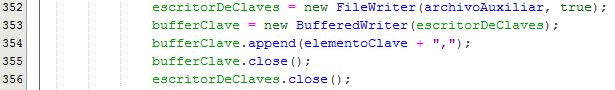
\includegraphics[height=3cm]{Imágenes/RaMe5.PNG}
    \caption{\textit{Escribe las claves en sus respectivo archivo auxiliar.}}
    \label{fig:RaMe5}
    \end{figure} 
     
    \item\textbf{sortAux}
    
    Con este método es posible finalizar el proceso de ordenamiento en cada iteración, pues este método el que lee las claves de los archivos auxiliares que recibe como primer parámetro y las escribe en las copia el archivo original creada desde un inicio, es decir el archivo que contenía las claves en desorden, es por eso que necesita recibir como parámetro el nombre de este archivo.
    
    \begin{figure}[h!]
    \centering
    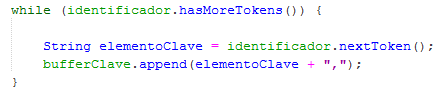
\includegraphics[height=4cm]{Imágenes/RaMe6.PNG}
    \caption{\textit{Método que concluye las iteraciones.}}
    \label{fig:RaMe6}
    \end{figure} 
    
    \item\textbf{recolectorDeBasura}
    
    La única función de este método  es eliminar archivos auxiliares en caso de que contengan claves, estos archivos son de ejecuciones anteriores y es necesario eliminarlos para evitar problemas con la ejecución actual.
    
    \begin{figure}[h!]
    \centering
    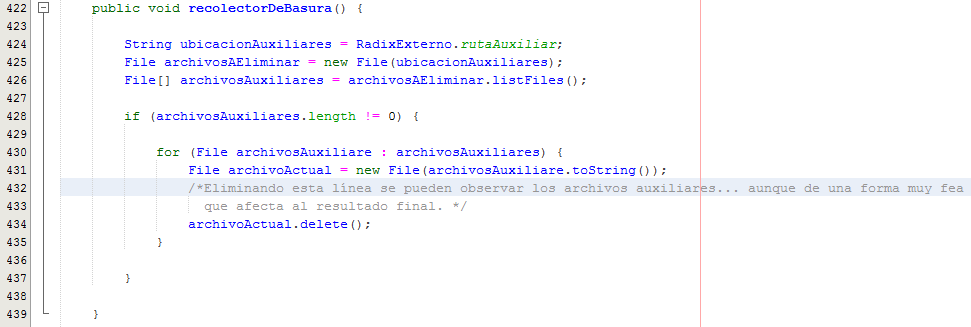
\includegraphics[height=6cm]{Imágenes/RaMe7.PNG}
    \caption{\textit{Elimina archivos auxiliares de ejecuciones anteriores.}}
    \label{fig:RaMe7}
    \end{figure}
    
    \pagebreak
    
    \item\textbf{impresionArchivo}
    
    Con apoyo de este método es posible escribir las claves correspondientes en el archivo que recibe como parámetro, este archivo será el que tenía las claves desordenadas y lo que se obtiene finalmente es un el archivo original pero con las claves ya ordenadas, es decir que con este método se finaliza el algoritmo.

    Es importante mencionar que cuando este método se utiliza en la primera iteración del algoritmo, obtiene las claves que han pasado por la primera iteración pero no necesariamente el archivo que recibe como parámetro este método tendrá la claves totalmente ordenadas.


    
    \begin{figure}[h!]
    \centering
    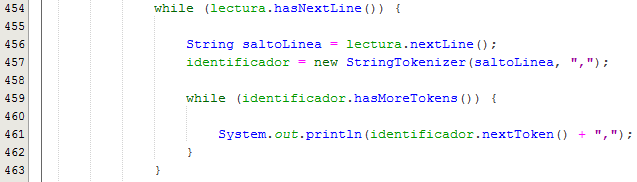
\includegraphics[height=5cm]{Imágenes/RaMe8.PNG}
    \caption{\textit{Vacía las claves ya ordenadas a la copia del archivo original.}}
    \label{fig:RaMe8}
    \end{figure} 
    
\end{itemize}

\pagebreak

\subsection{Simulación de la Mezcla Natural}

\noindent La programación de este método requiere consideraciones adicionales respecto a la generación de bloques:

\begin{enumerate}
\item Los bloques no son fijos y son de máximo tamaño, siguiendo un criterio ascendente o descendente.
\item Se requiere una comparación entre los elementos de cada arreglo; operación no realizable si no se dispone
de arreglos auxiliares que guarden los bloques contenidos en cada archivo.
\item Un mayor control de los bloques leídos y procesados es necesario para implementar efectivamente la escritura sobre los archivos.
\end{enumerate}

Con lo anterior en mente, se han añadido los siguientes atributos a la clase \textit{NaturalMix}:

\begin{figure}[h!]
    \centering
    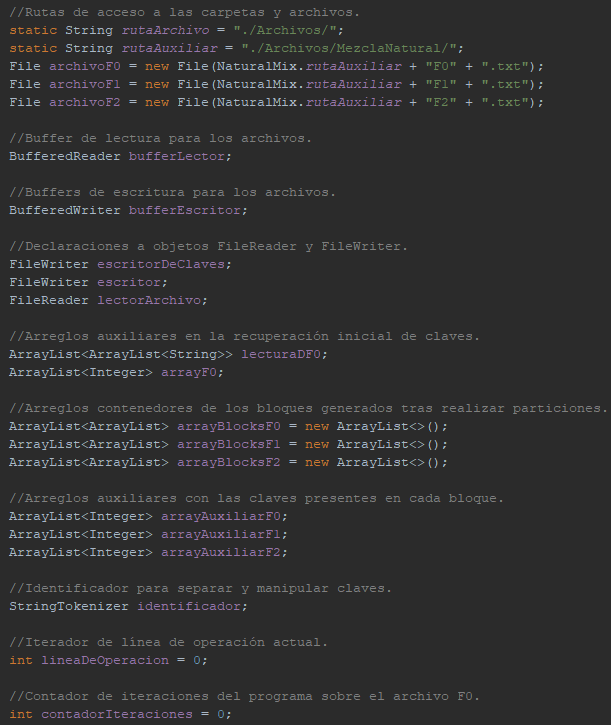
\includegraphics[height=13.2cm]{Imágenes/Natural1.png}
    \caption{\textit{Atributos de NaturalMix.}}
    \label{fig:Natural1}
    \end{figure} 
    
Los arreglos anidados \textbf{arrayBlocksFX} serán utilizados para el procesamiento de los bloques de claves presentes en los archivos, donde cada bloque es un arreglo con sus respectivas claves en orden ascendente o descendente, según corresponda. Así mismo, se inicializan archivo especiales para $F_{0}$, $F_{1}$ Y $F_{2}$. 

A continuación se dará un listado de los métodos de la clase. La documentación completa se encuentre en \textit{NaturalMix.java}

\begin{itemize}
\item \textbf{blockBuilder} es el método encargado de realizar las particiones sucesivas sobre las claves presentes en el archivo F0, previamente leídas y almacenadas en un arreglo, y realiza las particiones de máximo tamaño, de acuerdo al criterio seleccionado. El proceso se puede resumir en los siguientes pasos:

\begin{enumerate}
\item Se obtiene el primer elemento del arreglo y se coloca sobre un arreglo auxiliar que representa un bloque a insertar sobre $F_{1}$. Por medio de 2 variable de control, se comienza a iterar sobre el arreglo recibido y se añaden a la lista auxiliar los elementos que cumplan la condición máxima para cada partición.

\item Cuando se detecta que un elemento no comple el criterio establecido, se establece una primera partición que es cargada, en el caso particular del primer bloque procesado, sobre el arreglo arrayBlocksF2 por medio del método \textbf{addBlock} y por medio de la variable \textbf{bloqueActual}, se inicia una nueva partición que será escrita sobre $F_{2}$.

\item Finalmente, cualquier bloque que no haya sido tratado se añade a su respectivo arreglo, en caso de existir alguno. Finalmente, se imprimen las particiones almacenadas en \textbf{arrayBlocksF1} y \textbf{arrayBlocksF2} y se retorna la variable booleana \textbf{particionCreada}; que tendrá un valor $true$ en caso de que se haya realizado una partición válida sobre el arreglo recibido.


\end{enumerate}

\begin{figure}[h!]
    \centering
    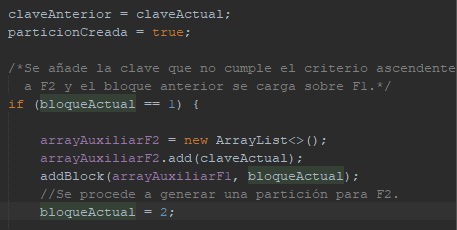
\includegraphics[height=5cm]{Imágenes/Natural2.png}
    \caption{\textit{Carga de los bloques de máximo tamaño.}}
    \label{fig:Natural2}
    \end{figure} 
    
\item El método \textbf{addBlock} se encarga de añadir un bloque de claves recibido a los arreglos \textbf{arrayBlocksF1} y \textbf{arrayBlocksF2}, según corresponda.

\begin{figure}[h!]
    \centering
    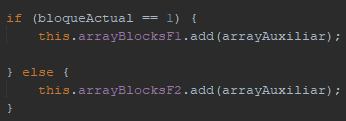
\includegraphics[height=3cm]{Imágenes/Natural3.png}
    \caption{\textit{Estructura del método.}}
    \label{fig:Natural3}
    \end{figure} 

\item El método \textbf{saltoLinea} añade 2 saltos de línea sobre el archivo introducido como parámetro. Este método es utilizado para separar las iteraciones almacenadas en cada uno de los archivos que ocupa \textit{MezclaNatural} durante su ejecución.

\begin{figure}[h!]
    \centering
    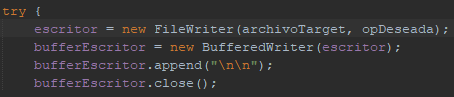
\includegraphics[height=2cm]{Imágenes/Natural4.png}
    \caption{\textit{Saltos de línea sobre el archivo introducido como parámetro.}}
    \label{fig:Natural4}
    \end{figure} 
    
\item El método \textbf{appendBlockToFile} se encarga de escribir un bloque de claves recibido como parámetro sobre el archivo seleccionado. Por defecto en la implementación realizado, la variable booleana \textbf{opDeseada} siempre tiene un valor \textit{true}. También se añade el método \textbf{appendKeyToFile} de Polifase como auxiliar en la generación inicial del arreglo contenedor de claves en $F_{0}$.

\begin{figure}[h!]
    \centering
    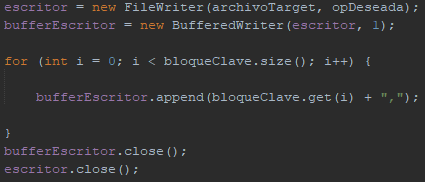
\includegraphics[height=5cm]{Imágenes/Natural5.png}
    \caption{\textit{Escritura de bloques sobre archivos.}}
    \label{fig:Natural5}
    \end{figure} 
    
    
\item \textbf{fileToArray} es una modificación del método \textbf{scanSuperKeys} adaptada exlcusivamente para su uso sobre la implementación de la Mezcla Natural. A diferencia del método anterior, este recibe directamente el archivo $F_{0}$ y tranforma la lectura de claves en un arreglo almacenado en \textbf{arrayBlocksF0}; el cual contiene las lecturas sucesivas de claves recuperadas tras cada iteración del programa. 

\begin{figure}[h!]
    \centering
    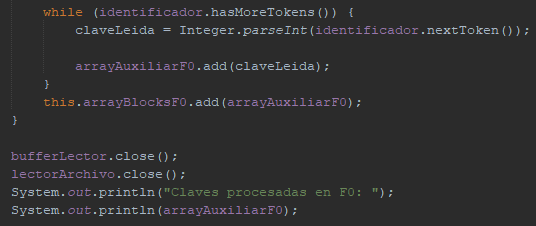
\includegraphics[height=5cm]{Imágenes/Natural6.png}
    \caption{\textit{Lecturas de claves en F0 almacenada en el arreglo de control de $F_{0}$.}}
    \label{fig:Natural6}
    \end{figure} 


\end{itemize}

\noindent Los métodos principales de la implementación son los siguientes:

\begin{itemize}
\item El método \textbf{mezclaNatural} recibe el nombre del archivo contenedor de claves y el criterio de ordenamiento seleccionado. Tras realizar un proceso de limpieza de los archivos de ejecuciones anteriores, se recupera el arreglo anidado con las superclaves  y, finalmente, se obtiene el arreglo con las claves, en este caso particular, numéricas para insertarlas en un archivo llamado \textbf{F0} en la carpeta \textit{Archivos $->$ MezclaNatural} por medio del método \textbf{appendKeyToFile}. Posteriormente, se añade al arreglo \textbf{arrayBlocksF0} el primer arreglo de claves leído en el archivo $F_{0}$.

Hecho lo anterior, se implementa un \textbf{switch} que, de acuerdo al criterio de ordenamiento seleccionado, realizará particiones sucesivas del contenido en $F_{0}$ almacenado; de acuerdo a la línea de operación actual del programa, y ejecutará el método \textbf{mixSort} encargado de procesar las particiones realizadas. Cuando el método \textbf{blockBuilder} informe que no se han realizado más particiones en $F_{0}$, el ciclo \textbf{while} implementado para repetir las operaciones anteriores se romperá y terminará la ejecución del ordenamiento.

\begin{figure}[h!]
    \centering
    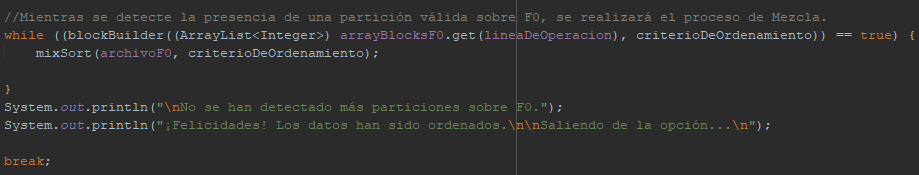
\includegraphics[height=3.5cm]{Imágenes/Natural7.png}
    \caption{\textit{Lecturas de claves en F0 almacenada en el arreglo de control de $F_{0}$.}}
    \label{fig:Natural7}
    \end{figure} 

\item \textbf{blockMerge} es el método encargado de realizar la mezcla o intercalado de los bloques presentes en los archivos $F_{1}$ Y $F_{2}$. En primer lugar, se inicializan listas auxiliares que representan un bloque de claves extraído sobre los archivos auxiliares. A continuación, se imprimen los bloques de claves presentes en $F_{1}$ Y $F_{2}$ y se declaran 2 variables booleanas que indican si existe un bloque para ser mezclado en los archivos auxiliares. A continuación, se recupera un bloque de cada arreglo representativo de los bloques presentes en $F_{1}$ Y $F_{2}$ y su contenido se añade a los arreglos secundarios declarados anteriormente.

\begin{figure}[h!]
    \centering
    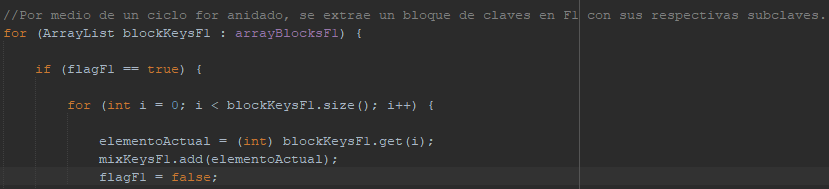
\includegraphics[height=3.5cm]{Imágenes/Natural8.png}
    \caption{\textit{Nótese que únicamente se recupera un único bloque para ser mezclado.}}
    \label{fig:Natural8}
    \end{figure} 
    
Realizado el procesado anterior, por medio de 2 ciclos \textbf{for-each} implementados, se recuperan las claves obtenidas por los arreglos secundarios y se almacenan en un arreglo llamado \textbf{mixedArray}. Finalmente, el arreglo obtenido es ordenado por medio del método \textbf{insertionSorting} de la clase \textit{Utilidades}, se imprime el resultado y se devuelve el arreglo obtenido.

\begin{figure}[h!]
    \centering
    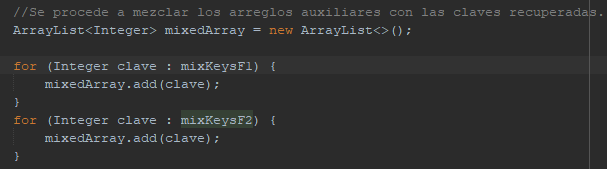
\includegraphics[height=3.5cm]{Imágenes/Natural9.png}
    \caption{\textit{Generación del arreglo mezclado que contiene 2 bloques de claves intercaladas.}}
    \label{fig:Natural9}
    \end{figure} 
    
\item El método \textbf{mixSort} se encarga de escribir sobre los archivos $F_{1}$ Y $F_{2}$ las particiones almacenadas en los arreglos de control \textbf{arrayBlocksF1} y \textbf{arrayBlocksF2}, respectivamente. Lo anterior es realizado por medio del método \textbf{forEach} definido para la clase \textit{ArrayList}.

\begin{figure}[h!]
    \centering
    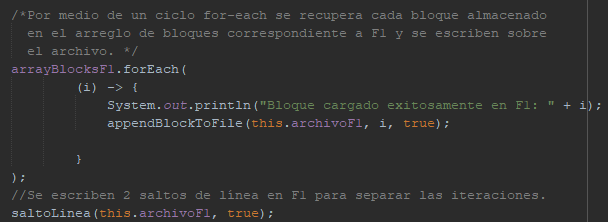
\includegraphics[height=4.5cm]{Imágenes/Natural10.png}
    \caption{\textit{Escritura de los particiones actuales sobre $F_{1}$ y $F_{2}$. Se insertan 2 saltos de línea tras cada escritura.}}
    \label{fig:Natural10}
    \end{figure} 
    
Una vez hecha la escritura, por medio de un ciclo \textbf{while} se proceden a añadir al archivo $F_{0}$ cada uno de los bloques intercalados por medio del método \textbf{blockMerge}. De esta forma, se realiza el intercalado de cada uno de los bloques y se realiza su escritura sobre $F_{0}$.

\begin{figure}[h!]
    \centering
    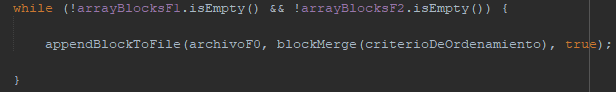
\includegraphics[height=2cm]{Imágenes/Natural11.png}
    \caption{\textit{Proceso de escritura de los bloques mezclados sobre $F_{0}$, siempre y cuando ambos arreglos tengan bloques válidos por intercalar.}}
    \label{fig:Natural11}
    \end{figure} 
    
\pagebreak

Finalmente, cualquier bloque que no hibiese sido añadido a $F_{0}$. es añadido haciendo una verificación sobre los arreglos de control de $F_{1}$ y $F_{2}$. Luego, se incrementa en 2 unidades la línea de operación actual de la ejecución y se incrementa el contador de iteraciones realizadas. El método termine imprimiendo un mensaje de estado, limpia el arreglo de control de $F_{0}$ e inicia un nueva lectura sobre $F_{0}$. Es importante señalar el papel que la variable \textbf{lineaDeOperacion} tiene debido a que, tras inspeccionar nuevamente  $F_{0}$, el arreglo \textbf{arrayBlocksF0} tendrá 3 índices en su interior: la iteración original, los saltos de línea agregados, y escritura realizada de las claves mezcladas. Por medio del incremente en 2 unidades de esta variable, se accede correctamente a las escrituras sucesivas que se realizan en $F_{0}$; como se muestra en [\ref{fig:Natural12}].
    

\end{itemize}

\begin{figure}[h!]
    \centering
    \includegraphics[height=4cm]{Imágenes/Natural12.png}
    \caption{\textit{Procedimiento final del método.}}
    \label{fig:Natural12}
    \end{figure} 
    
\section{Mezcla Natural no numérica}

\noindent El ordenamiento de claves no numéricas contiene diferencias con respecto al enfoque numérico, en un caso semejante al de Polifase. Su implementación se encuentre contenida sobre otra clase que hereda directamente de \textit{NaturalMix}: a esta clase se le ha denominado \textit{NaturalMixStrings}. A continuación se enlistan los cambios realizados:

\begin{itemize}
\item En el método \textbf{mezclaNatural} ahora se recuperan claves no numéricas de acuerdo al campo seleccionado: nombre o apellido.
\item Los métodos \textbf{blockBuilder}, \textbf{blockMerge}, \textbf{appendBlockToFile} y \textbf{appendKeyToFile} han sido adaptados para recibir y procesar claves de tipo String.
\item Se han sobreescrito los métodos \textbf{mixSort} y \textbf{fileToArray} para que operen adecuadamente al leer claves String y el proceso de intercalado y ordenamiento interno funcione adecuadamente.
\end{itemize}



\section{Pruebas de funcionamiento y rendimiento}

\noindent A continuación se mostrarán capturas de pantalla del funcionamiento del programa haciendo uso de diversos criterios y utilizando un archivo de 100 claves, como puede verse a continuación:

\begin{figure}[h!]
    \centering
    \includegraphics[height=8.9cm]{Imágenes/Func1.png}
    \caption{\textit{Vista previo del archivo con 100 claves a utilizar.}}
    \label{fig:Func1}
    \end{figure} 

\begin{figure}[h!]
    \centering
    \includegraphics[height=8.9cm]{Imágenes/Func2.png}
    \caption{\textit{Ejecución de Polifase con las opciones mostradas en la captura.}}
    \label{fig:Func2}
    \end{figure} 
    
\pagebreak

\begin{figure}[h!]
    \centering
    \includegraphics[height=8.9cm]{Imágenes/Func3.png}
    \caption{\textit{Generación de los bloques de tamaño fijo.}}
    \label{fig:Func3}
    \end{figure} 

\begin{figure}[h!]
    \centering
    \includegraphics[height=10cm]{Imágenes/Func4.png}
    \caption{\textit{Proceso de intercalado realizado con los bloques recuperados.}}
    \label{fig:Func4}
    \end{figure} 
    
    \begin{figure}[h!]
    \centering
    \includegraphics[height=5.5cm]{Imágenes/Func5.png}
    \caption{\textit{Resultado obtenido.}}
    \label{fig:Func5}
    \end{figure}
    




\newpage\section{Conclusiones}



\begin{itemize}
    \item \textbf{López Lara Marco Antonio}
    
    Debido a que algunas partes esenciales de nuestro codigo no funcionaban de la manera correcta se hizo necesaria una investigacion de estructura de datos en especifico del ordenamiento de datos, en este proyecto nuestra prioridad era el manejo de datos o archivos .TXTen java debido a nuestro equipo tenia experiencia con el uso de dichos archivos pero muy poca en el lenguaje de programacion JAVA.
    
    El uso de archivos es muy relevante en el proyecto debido a su importancia ya que en ellos se guardaran nuestras claves, y en algunas cuestiones será necesario de otros archivos para almacenar nuestras claves que seran ordenas y guardas o sobreescribir en el archivo.
    
    En el proyecto vi el uso de lo anteriormente aprendido en la clase, también fue de mucha ayuda para poder entender mejor la polifase, mezcla natural, radix externo ya que los tres yo no los había entendido hasta que con la ayuda de del proyecto y de mis compañeros lo entendí.
    
    Me llevo nuevos conocimientos de algunas ectre ellas es el uso de Try para las excepciones de nuestras claves y siendo que si existe una excepcion no cause que nuestro programa no siga avanzando.
    
    
    \item \textbf{Olivera Martínez Jenyffer Brigitte}
    
    A medida que se avanzaba en el proyecto era necesario ir investigando distintos aspecto en relación con el manejo archivos en java. Aspecto completamente nuevo en el lenguaje que se está aprendiendo y el paradigma orientado a objetos. Si bien este aspecto representó un primer acercamiento al manejo de archivos en Java, crea una base para el desarrollo de conocimientos a futuro, pues al momento  en el que en el curso deban tratarse archivos no se llegará con la mente el blanco.

    El manejo de archivos es relevante no solo para la cuestión de ordenamiento externo, muchas veces al momento de resolver problemas en programación los archivos será la primer fuente de información para la solución de algún problema  específico, además de optimizar la gestión de información, aspecto que hace a los archivos una herramienta fundamental para cualquier programador.
    
    Al igual que con el manejo de archivos, se pusieron en práctica muchos de los conocimientos adquiridos a partir de los temas vistos en clase y se profundizó en ellos, lo que contribuye a aclarar cualquier aspecto que no haya sido entendido.
    
    Otro aspecto relevante en cuanto a los elementos utilizados en el proyecto son las excepciones, pues se debe ser consciente de que pueden llegar a aparecer ella corrida de algún programa y es necesario saber las acciones que deben tomarse ante ellas.
    
    De hicieron notar las diferencias entre los algoritmos que se emplearon, cada uno tiene similitudes y diferencias, por ejemplo, el hecho de que todos estos algoritmos están basados en la estrategia “divide y vencerás”, no significa que hagan la división de la información de la misma manera, pues cada algoritmo emplea sus propios métodos. Así mismo los criterios que utiliza cada algoritmo son distintos: Poliface establece bloques de tamaño fijo y emplea algún algoritmo de ordenamiento interno, Mezcla Equilibrada establece bloques ordenados y Radix externo emplea un criterio de ordenamiento distinto, pues toma en cuenta dígitos significativos, cosa que no para en ninguno de los otros dos algoritmos. 
    
    Sin lugar a duda este proyecto contribuye de manera significativa a el desarrollo de nuevos conocimientos e implementaciones de los algoritmos y antecedentes. En cuanto al trabajo en equipo, el proyecto hace notar las diferencias en cuanto al ritmo de trabajo de cada individuo y resalta la importancia de las contribuciones de equipo, pues pese a las diferencias que puedan existir, el trabajo en equipo reúne las habilidades de cada integrante para un fin común y de esta manera desarrollar más habilidades y apreciar las aportaciones que cada integrante puede hacer.
    
    Para concluir en mi experiencia los objetivos del proyecto fueron los correctos y fueron llevados acabo ya que pienso que nuestro equipo se lleva bastantes conocimientos extras así como el uso de latex y algunas cuestiones de java, para mi el proyecto es de gran ayuda en mi formación como ingeniero ya que con ello puedo ver las utilidades de los conocmientos que voy adquiriendo y que verdaderamente son usados y utiles.

    
    \item \textbf{Téllez González Jorge Luis}
    
    El primer proyecto realizado para el curso de EDA II representa una culminación del desarrollo de habilidades que cada uno de los integrantes ha tenido que desarrollar a lo largo de las prácticas de laboratorio, debido a que muchos de los conceptos usados en las implementaciones programadas requieren el manejo, por citar algunos ejemplos, de clases como \textit{ArrayList}. Por otra parte, el desarrollo de habilidades de manejo de archivos externos fue una componente interesante de estudiar y aplicar; ya que en mi experiencia previa de Java únicamente llegué a leer contenido de un archivo. En cambio, en el proyecto me vi forzado a llevar más allá esta habilidad y aprender a hacer un manejo eficiente de los procesos de entrada/salida sobre archivos.
    
    Entre los puntos más relevantes que puedo comentar de la experiencia obtenida se encuentran los siguientes:
    
    
\begin{itemize}
\item La primer gran dificultad fue, evidentemente, aprender a manejar los archivos \textit{File}, así como todas las clases que operan sobre ellos. En un inicio fue una experiencia tremendamente frustrante y sin demasiados avances; especialmente al experiementar con la escritura sobre archivos. Me tomó una cantidad considerable de tiempo leer la documentación proporcionada por Oracle y experimentar en \textbf{NetBeans}. Por supuesto, el esfuerzo rindió sus frutos y el manejo de los procesos de lectura/escritura se volvió una tarea mucho más sencilla e intuitiva.

\item El primer método programado fue la simulación de Radix-Externo. Sin embargo, fue escrito considerando únicamente claves numéricas simples. Idear e implementar la solución a la lectura de las superclaves con 3 campos fue un obstáculo que no pudimos sortear efectivamente hasta que, experimentando y estudiando los ejemplos de la clase teórica escribí el método \textbf{scanSuperKeys}, el cual es vital en todas las implementaciones escritas y representa, por su importancia en la lectura inicial, uno de los métodos más importantes del proyecto. 

\item El método de ordenamiento que, considero, fue el más complicado de implementar fue la Mezcla Natural. El enfoque de particiones máximas requirió un mayor tiempo de abstracción a diferencia de Polifase, así como un control más elevado de los bloques escritos en cada archivo: por ello, se implementaron arreglos de control para tener un control efectivo de los datos entrantes y salientes dentro de los archivos utilizados por el programa.

\end{itemize}

La programación de cada uno de los métodos, sin duda, fue una experiencia muy retadora y frustrante en ocasiones. Después de sortear una gran cantidad de excepciones \textit{nullPointer} o relacionadas con los índices de los arreglos, el resultado final en cada implementación refleja un proceso de \textit{sudor y sangre}: una satisfacción que solo una persona del área puede comprender.

La experiencia final es una gran cantidad de conocimiento adquirido. Por supuesto, el trabajo en equipo es importante y la conclusión del proyecto no hubiese sido posible con una única persona. Esto es un importante recordatorio de la importancia del trabajo en equipo en la Ingeniería en cualquiera de sus campos de acción. Tengo la certeza que toda la experiencia obtenida será invaluable durante el desarrollo del resto del curso; pese a que la situación actual en México ha afectado la dinámica de toda la \textbf{UNAM}. Sin embargo, no nos detenemos y seguimos trabajando pese a todas las adversidades a las que nos enfrentemos.
    
    
    


\end{itemize}

            \nocite{Cairo}
            \nocite{Ceballos}
            \nocite{Cormen}
            \nocite{1}
            \nocite{Joyanes}
            \nocite{McConnell}
            \nocite{Skiena}
	        \bibliographystyle{apalike}
            \bibliography{Libros.bib}

\centering \small Los créditos de las fotografías pertenecen a sus respectivos autores. ©

\centering\vspace*{\fill} \LaTeX{}
\end{document}
